\documentclass[11pt,a4paper,]{article}
\usepackage{lmodern}

\usepackage{amssymb,amsmath}
\usepackage{ifxetex,ifluatex}
\usepackage{fixltx2e} % provides \textsubscript
\ifnum 0\ifxetex 1\fi\ifluatex 1\fi=0 % if pdftex
  \usepackage[T1]{fontenc}
  \usepackage[utf8]{inputenc}
\else % if luatex or xelatex
  \usepackage{unicode-math}
  \defaultfontfeatures{Ligatures=TeX,Scale=MatchLowercase}
\fi
% use upquote if available, for straight quotes in verbatim environments
\IfFileExists{upquote.sty}{\usepackage{upquote}}{}
% use microtype if available
\IfFileExists{microtype.sty}{%
\usepackage[]{microtype}
\UseMicrotypeSet[protrusion]{basicmath} % disable protrusion for tt fonts
}{}
\PassOptionsToPackage{hyphens}{url} % url is loaded by hyperref
\usepackage[unicode=true]{hyperref}
\hypersetup{
            pdftitle={COVID 19 Report},
            pdfborder={0 0 0},
            breaklinks=true}
\urlstyle{same}  % don't use monospace font for urls
\usepackage{geometry}
\geometry{a4paper, centering, text={16cm,24cm}}
\usepackage[style=authoryear-comp,]{biblatex}
\addbibresource{references.bib}
\usepackage{longtable,booktabs}
% Fix footnotes in tables (requires footnote package)
\IfFileExists{footnote.sty}{\usepackage{footnote}\makesavenoteenv{long table}}{}
\usepackage{graphicx,grffile}
\makeatletter
\def\maxwidth{\ifdim\Gin@nat@width>\linewidth\linewidth\else\Gin@nat@width\fi}
\def\maxheight{\ifdim\Gin@nat@height>\textheight\textheight\else\Gin@nat@height\fi}
\makeatother
% Scale images if necessary, so that they will not overflow the page
% margins by default, and it is still possible to overwrite the defaults
% using explicit options in \includegraphics[width, height, ...]{}
\setkeys{Gin}{width=\maxwidth,height=\maxheight,keepaspectratio}
\IfFileExists{parskip.sty}{%
\usepackage{parskip}
}{% else
\setlength{\parindent}{0pt}
\setlength{\parskip}{6pt plus 2pt minus 1pt}
}
\setlength{\emergencystretch}{3em}  % prevent overfull lines
\providecommand{\tightlist}{%
  \setlength{\itemsep}{0pt}\setlength{\parskip}{0pt}}
\setcounter{secnumdepth}{5}

% set default figure placement to htbp
\makeatletter
\def\fps@figure{htbp}
\makeatother


\title{COVID 19 Report}

%% MONASH STUFF

%% CAPTIONS
\RequirePackage{caption}
\DeclareCaptionStyle{italic}[justification=centering]
 {labelfont={bf},textfont={it},labelsep=colon}
\captionsetup[figure]{style=italic,format=hang,singlelinecheck=true}
\captionsetup[table]{style=italic,format=hang,singlelinecheck=true}


%% FONT
\RequirePackage{bera}
\RequirePackage[charter,expert,sfscaled]{mathdesign}
\RequirePackage{fontawesome}

%% HEADERS AND FOOTERS
\RequirePackage{fancyhdr}
\pagestyle{fancy}
\rfoot{\Large\sffamily\raisebox{-0.1cm}{\textbf{\thepage}}}
\makeatletter
\lhead{\textsf{\expandafter{\@title}}}
\makeatother
\rhead{}
\cfoot{}
\setlength{\headheight}{15pt}
\renewcommand{\headrulewidth}{0.4pt}
\renewcommand{\footrulewidth}{0.4pt}
\fancypagestyle{plain}{%
\fancyhf{} % clear all header and footer fields
\fancyfoot[C]{\sffamily\thepage} % except the center
\renewcommand{\headrulewidth}{0pt}
\renewcommand{\footrulewidth}{0pt}}

%% MATHS
\RequirePackage{bm,amsmath}
\allowdisplaybreaks

%% GRAPHICS
\RequirePackage{graphicx}
\setcounter{topnumber}{2}
\setcounter{bottomnumber}{2}
\setcounter{totalnumber}{4}
\renewcommand{\topfraction}{0.85}
\renewcommand{\bottomfraction}{0.85}
\renewcommand{\textfraction}{0.15}
\renewcommand{\floatpagefraction}{0.8}


%\RequirePackage[section]{placeins}

%% SECTION TITLES


%% SECTION TITLES (NEW: Changing sections and subsections color)
\RequirePackage[compact,sf,bf]{titlesec}
\titleformat*{\section}{\Large\sf\bfseries\color[rgb]{0.8, 0.7, 0.1 }}
\titleformat*{\subsection}{\large\sf\bfseries\color[rgb]{0.8, 0.7, 0.1 }}
\titleformat*{\subsubsection}{\sf\bfseries\color[rgb]{0.8, 0.7, 0.1 }}
\titlespacing{\section}{0pt}{2ex}{.5ex}
\titlespacing{\subsection}{0pt}{1.5ex}{0ex}
\titlespacing{\subsubsection}{0pt}{.5ex}{0ex}


%% TITLE PAGE
\def\Date{\number\day}
\def\Month{\ifcase\month\or
 January\or February\or March\or April\or May\or June\or
 July\or August\or September\or October\or November\or December\fi}
\def\Year{\number\year}

%% LINE AND PAGE BREAKING
\sloppy
\clubpenalty = 10000
\widowpenalty = 10000
\brokenpenalty = 10000
\RequirePackage{microtype}

%% PARAGRAPH BREAKS
\setlength{\parskip}{1.4ex}
\setlength{\parindent}{0em}

%% HYPERLINKS
\RequirePackage{xcolor} % Needed for links
\definecolor{darkblue}{rgb}{0,0,.6}
\RequirePackage{url}

\makeatletter
\@ifpackageloaded{hyperref}{}{\RequirePackage{hyperref}}
\makeatother
\hypersetup{
     citecolor=0 0 0,
     breaklinks=true,
     bookmarksopen=true,
     bookmarksnumbered=true,
     linkcolor=darkblue,
     urlcolor=blue,
     citecolor=darkblue,
     colorlinks=true}

\usepackage[showonlyrefs]{mathtools}
\usepackage[no-weekday]{eukdate}

%% BIBLIOGRAPHY

\makeatletter
\@ifpackageloaded{biblatex}{}{\usepackage[style=authoryear-comp, backend=biber, natbib=true]{biblatex}}
\makeatother
\ExecuteBibliographyOptions{bibencoding=utf8,minnames=1,maxnames=3, maxbibnames=99,dashed=false,terseinits=true,giveninits=true,uniquename=false,uniquelist=false,doi=false, isbn=false,url=true,sortcites=false}

\DeclareFieldFormat{url}{\texttt{\url{#1}}}
\DeclareFieldFormat[article]{pages}{#1}
\DeclareFieldFormat[inproceedings]{pages}{\lowercase{pp.}#1}
\DeclareFieldFormat[incollection]{pages}{\lowercase{pp.}#1}
\DeclareFieldFormat[article]{volume}{\mkbibbold{#1}}
\DeclareFieldFormat[article]{number}{\mkbibparens{#1}}
\DeclareFieldFormat[article]{title}{\MakeCapital{#1}}
\DeclareFieldFormat[article]{url}{}
%\DeclareFieldFormat[book]{url}{}
%\DeclareFieldFormat[inbook]{url}{}
%\DeclareFieldFormat[incollection]{url}{}
%\DeclareFieldFormat[inproceedings]{url}{}
\DeclareFieldFormat[inproceedings]{title}{#1}
\DeclareFieldFormat{shorthandwidth}{#1}
%\DeclareFieldFormat{extrayear}{}
% No dot before number of articles
\usepackage{xpatch}
\xpatchbibmacro{volume+number+eid}{\setunit*{\adddot}}{}{}{}
% Remove In: for an article.
\renewbibmacro{in:}{%
  \ifentrytype{article}{}{%
  \printtext{\bibstring{in}\intitlepunct}}}

\AtEveryBibitem{\clearfield{month}}
\AtEveryCitekey{\clearfield{month}}

\makeatletter
\DeclareDelimFormat[cbx@textcite]{nameyeardelim}{\addspace}
\makeatother

\author{\sf\Large\textbf{ Lintian Zhang}\\ {\sf\large Bachelor of Accounting\\[0.5cm]} \sf\Large\textbf{ Arthur Andersen Widjaya}\\ {\sf\large Bachelor of Accounting\\[0.5cm]} \sf\Large\textbf{ Hanchen Wang}\\ {\sf\large Bachelor of Finance\\[0.5cm]} \sf\Large\textbf{ Ying Zou}\\ {\sf\large Bachelor of Economics\\[0.5cm]}}

\date{\sf\Date~\Month~\Year}
\makeatletter
\lfoot{\sf Zhang, Widjaya, Wang, Zou: \@date}
\makeatother


%%%% PAGE STYLE FOR FRONT PAGE OF REPORTS

\makeatletter
\def\organization#1{\gdef\@organization{#1}}
\def\telephone#1{\gdef\@telephone{#1}}
\def\email#1{\gdef\@email{#1}}
\makeatother
  \organization{Australian Government COVID19}

  \def\name{Team Amazing}

  \telephone{(03) 9905 2478}

  \email{questions@company.com}                 %NEW: New email addresss

\def\webaddress{\url{http://company.com/stats/consulting/}} %NEW: URl
\def\abn{12 377 614 630}                                    % NEW: ABN
\def\logo{\includegraphics[width=6cm]{Figures/logo}}  %NEW: Changing logo
\def\extraspace{\vspace*{1.6cm}}
\makeatletter
\def\contactdetails{\faicon{phone} & \@telephone \\
                    \faicon{envelope} & \@email}
\makeatother

%%%% FRONT PAGE OF REPORTS

\def\reporttype{Report for}

\long\def\front#1#2#3{
\newpage
\begin{singlespacing}
\thispagestyle{empty}
\vspace*{-1.4cm}
\hspace*{-1.4cm}
\hbox to 16cm{
  \hbox to 6.5cm{\vbox to 14cm{\vbox to 25cm{
    \logo
    \vfill
    \parbox{6.3cm}{\raggedright
      \sf\color[rgb]{0.8, 0.7, 0.1 }    % NEW color 
      {\large\textbf{\name}}\par
      \vspace{.7cm}
      \tabcolsep=0.12cm\sf\small
      \begin{tabular}{@{}ll@{}}\contactdetails
      \end{tabular}
      \vspace*{0.3cm}\par
      ABN: \abn\par
    }
  }\vss}\hss}
  \hspace*{0.2cm}
  \hbox to 1cm{\vbox to 14cm{\rule{4pt}{26.8cm}\vss}\hss\hfill}  %NEW: Thicker line
  \hbox to 10cm{\vbox to 14cm{\vbox to 25cm{   
      \vspace*{3cm}\sf\raggedright
      \parbox{11cm}{\sf\raggedright\baselineskip=1.2cm
         \fontsize{24.88}{30}\color[rgb]{0, 0.29, 0.55}\sf\textbf{#1}}   % NEW: title color blue
      \par
      \vfill
      \large
      \vbox{\parskip=0.8cm #2}\par
      \vspace*{2cm}\par
      \reporttype\\[0.3cm]
      \hbox{#3}%\\[2cm]\
      \vspace*{1cm}
      {\large\sf\textbf{\Date~\Month~\Year}}
   }\vss}
  }}
\end{singlespacing}
\newpage
}

\makeatletter
\def\titlepage{\front{\expandafter{\@title}}{\@author}{\@organization}}
\makeatother

\usepackage{setspace}
\setstretch{1.5}

%% Any special functions or other packages can be loaded here.
\usepackage{float} \floatplacement{figure}{H} \floatplacement{table}{H}
\usepackage{booktabs}
\usepackage{longtable}
\usepackage{array}
\usepackage{multirow}
\usepackage{wrapfig}
\usepackage{float}
\usepackage{colortbl}
\usepackage{pdflscape}
\usepackage{tabu}
\usepackage{threeparttable}
\usepackage{threeparttablex}
\usepackage[normalem]{ulem}
\usepackage{makecell}
\usepackage{xcolor}


\begin{document}
\titlepage

\hypertarget{introduction}{%
\section{Introduction}\label{introduction}}

\href{https://www.covid19data.com.au}{Covid19 data Australia} is the source where we get all the data. We are analyzing the cases as in 18 of May 2021 where we download all the data needed. We divided our analysis to 4 part, firstly we are going to talk about the total cases within the last 28 days in Australia, secondly we are going to talk about the cases we also analyze the how many people recover due to the disease, after looking at the transmission sources in Australia, and lastly we talked about the vaccination program which starts from February to 18 May.

The purpose of this report is to analyze how well Australia is handling the pandemic, we decided to do this because we all aware that the pandemic is keep on heating from time to time so it's very important for us international students who is studying in Australia be aware of what is happening in Australia.

\section*{Total cases in Australia}

\hypertarget{total-covid-19-cases-from-each-state-in-the-last-28-days}{%
\section{Total COVID 19 cases from each state in the last 28 days}\label{total-covid-19-cases-from-each-state-in-the-last-28-days}}

\begin{table}

\caption{\label{tab:table1}Total cases in 28 days}
\centering
\begin{tabular}[t]{l|r}
\hline
state & total\\
\hline
NSW & 211\\
\hline
SA & 71\\
\hline
QLD & 59\\
\hline
NT & 57\\
\hline
VIC & 53\\
\hline
WA & 50\\
\hline
ACT & 1\\
\hline
TAS & 0\\
\hline
\end{tabular}
\end{table}

\hypertarget{analysis}{%
\subsection{Analysis}\label{analysis}}

table \ref{tab:table1} shows the total number of COVID 19 cases from all the states in Australia in the last 28 days. It clearly shows that in the last 28 days New South Wales (NSW) has added the most number of cases with total of 211 cases. Compared to other states they only at 50's cases with Australian Capital Territory (ACT) and Tasmania (TAS) only added 1 and 0 cases. It reflects that NSW has been struggling. The data was downloaded as in 18 of May 2021, they really need to increase their attention in order to contain the virus outbreak.

\hypertarget{highest-and-lowest-covid-19-cases-in-australia}{%
\section{Highest and lowest COVID 19 cases in Australia}\label{highest-and-lowest-covid-19-cases-in-australia}}

\begin{figure}
\centering
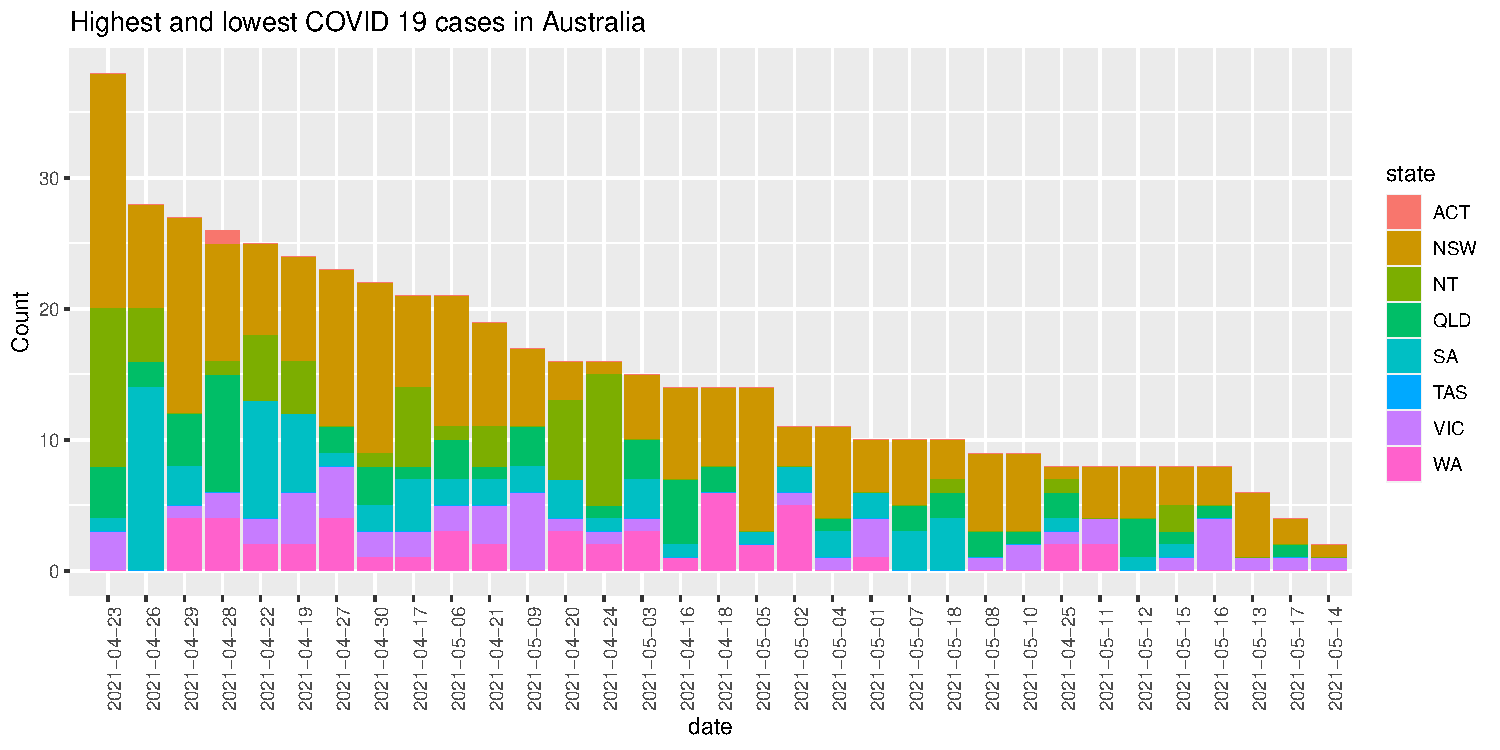
\includegraphics{report_files/figure-latex/figref1-1.pdf}
\caption{\label{fig:figref1}Highest and lowest COVID 19 cases in Australia}
\end{figure}

\hypertarget{analysis-1}{%
\subsection{Analysis}\label{analysis-1}}

Figure \ref{fig:figref1} showing the highest to lowest cases of COVID 19 the X axis acts recorded the date on when the case was recorded. At glance at the 23 of April 2021 the day where Australia adds the higest total cases with NSW is the highest contributor, and the lowest cases was recorded at 14 May 2021.

\hypertarget{covid-19-cases-in-australia-in-the-last-28-days}{%
\section{COVID 19 cases in Australia in the last 28 days}\label{covid-19-cases-in-australia-in-the-last-28-days}}

\begin{figure}
\centering
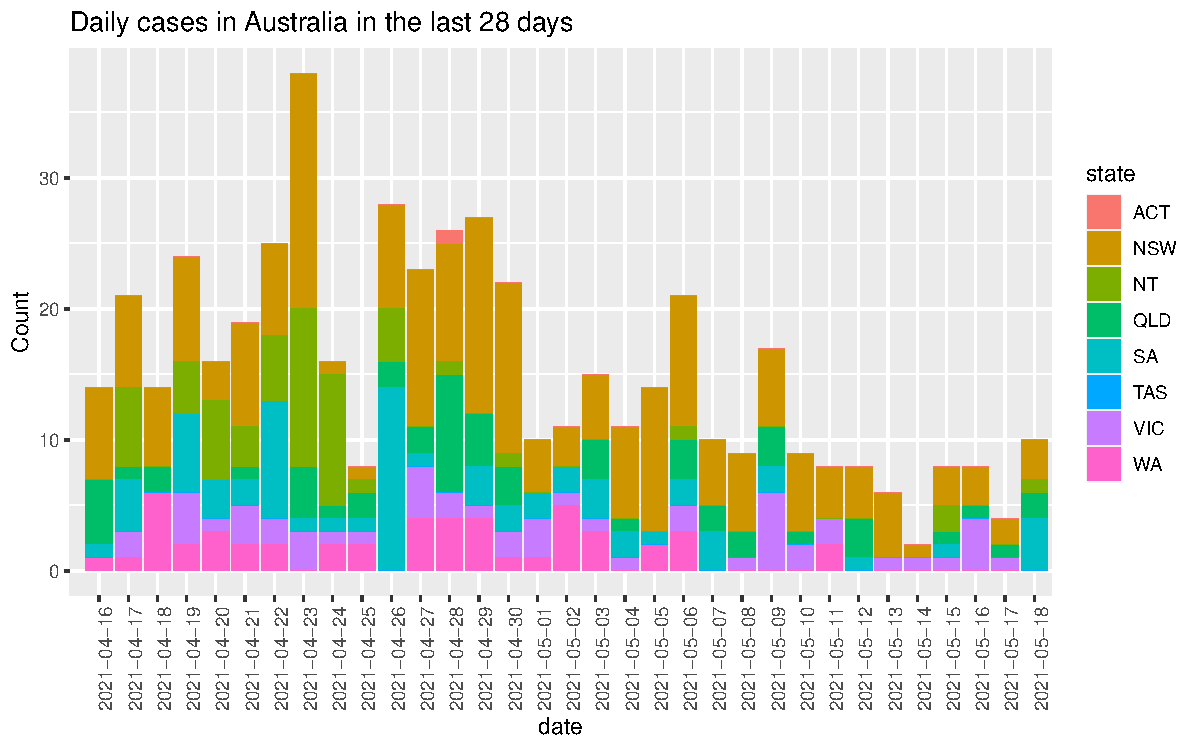
\includegraphics{report_files/figure-latex/figref2-1.pdf}
\caption{\label{fig:figref2}Daily cases in Australia in the last 28 days}
\end{figure}

\hypertarget{analysis-2}{%
\subsection{Analysis}\label{analysis-2}}

\ref{fig:figref2} showing the COVID 19 cases trends from 16 of April to 18 of May 2021. During the first few weeks the cases has rises and reaches it's peak on the 22 April 2021. 2 days later it drops and suddenly there has been an increase again. But overall during the last 28 days Australia has shown a great way to contain the outbreak on the first week which showing the efficiency of the government rules and regulation.

\section*{Recovery}

\hypertarget{recovery-count}{%
\section{Recovery count}\label{recovery-count}}

\begin{figure}
\centering
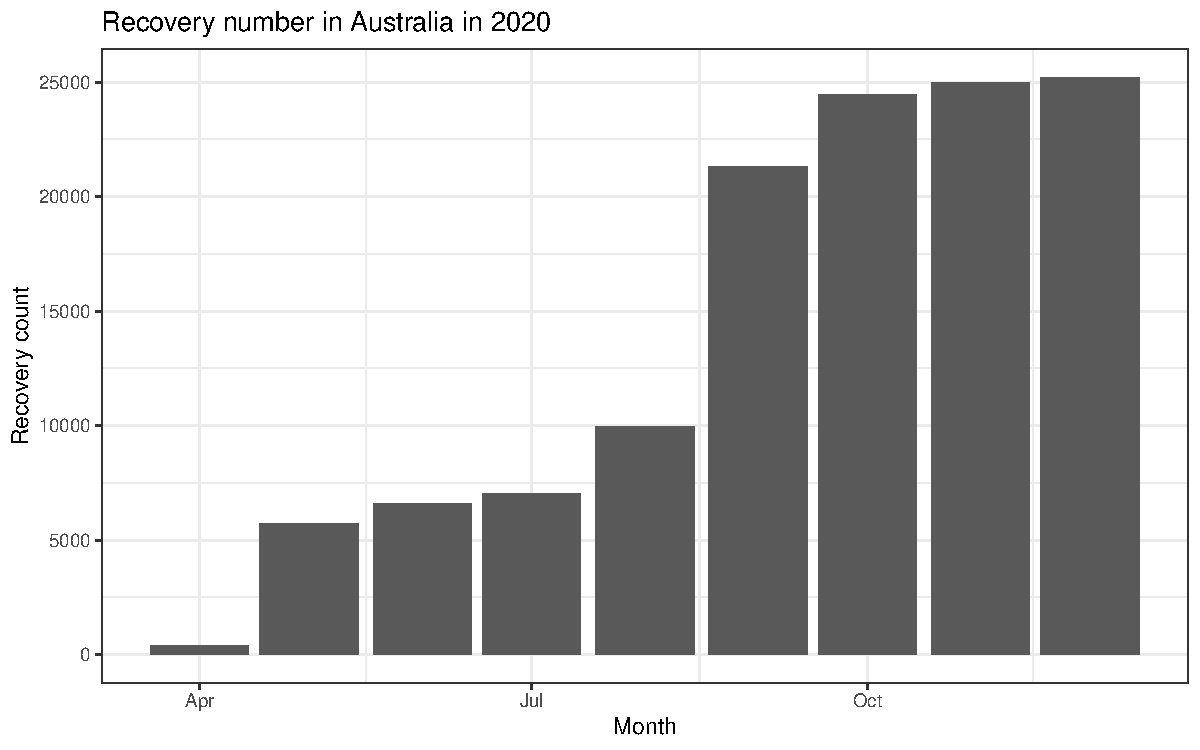
\includegraphics{report_files/figure-latex/figrec1-1.pdf}
\caption{\label{fig:figrec1}Recovery number in Australia in 2020}
\end{figure}

\hypertarget{analysis-3}{%
\subsection{Analysis}\label{analysis-3}}

Figure \ref{fig:figrec1} shows that the number of recoveries from 2020.3 to 2021.5. It is not hard to find there was a slow climb before 2020.07(248918), after which a double recoveries appeared which is referred to the focus and good care on COVID-19 among countries. Then the number kept constant with some fluctuation.

\hypertarget{recovery-rate}{%
\section{Recovery Rate}\label{recovery-rate}}

\begin{figure}
\centering
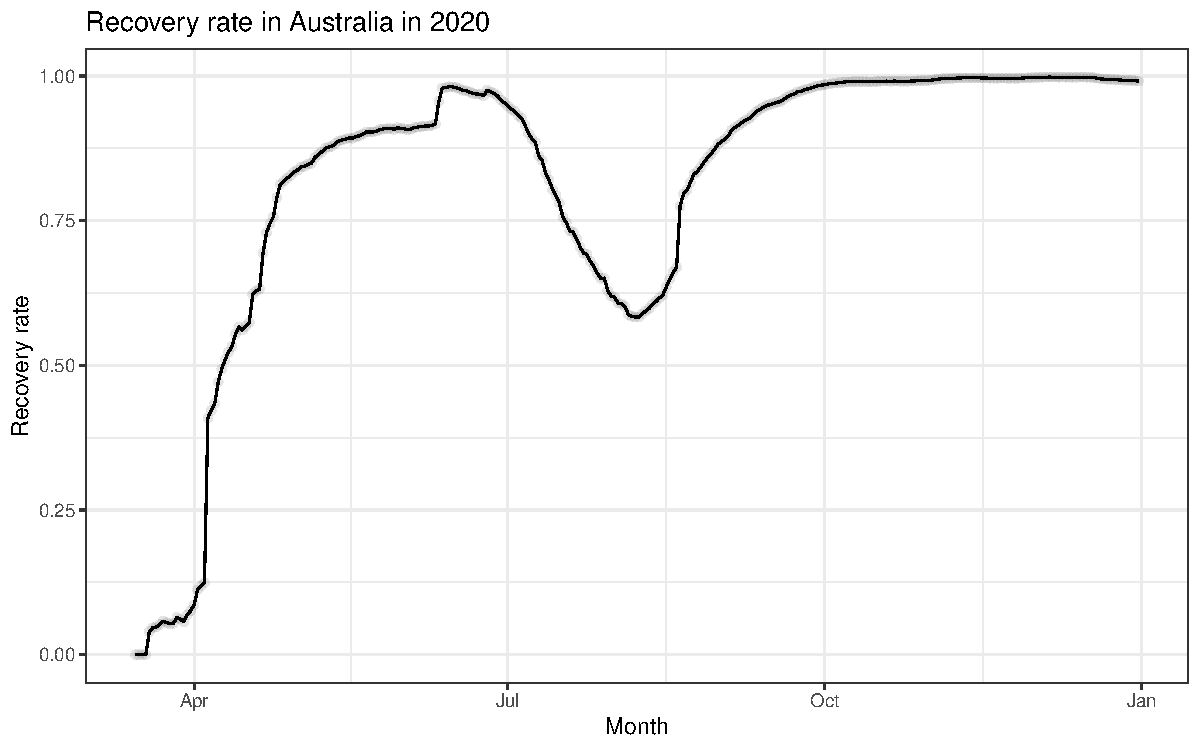
\includegraphics{report_files/figure-latex/figrec2-1.pdf}
\caption{\label{fig:figrec2}Recovery rate in Australia in 2020}
\end{figure}

\hypertarget{analysis-4}{%
\subsection{Analysis}\label{analysis-4}}

Figure \ref{fig:figrec2} shows that the total recovery rate had an increase before 2020.6(95\%), and a downward trend happened due to the decreasing active cases as well as increasing recoveries. However, the recovery rate continued to climbing from 2020.8(71\%) and reached at almost 99\% after 2020.11 until now.The main reason that the rate kept increasing steep is that the government did control the virus situation to some extend, the less active cases, the higher rate.

\hypertarget{recovery-death-ratio}{%
\section{Recovery-death ratio}\label{recovery-death-ratio}}

\begin{figure}
\centering
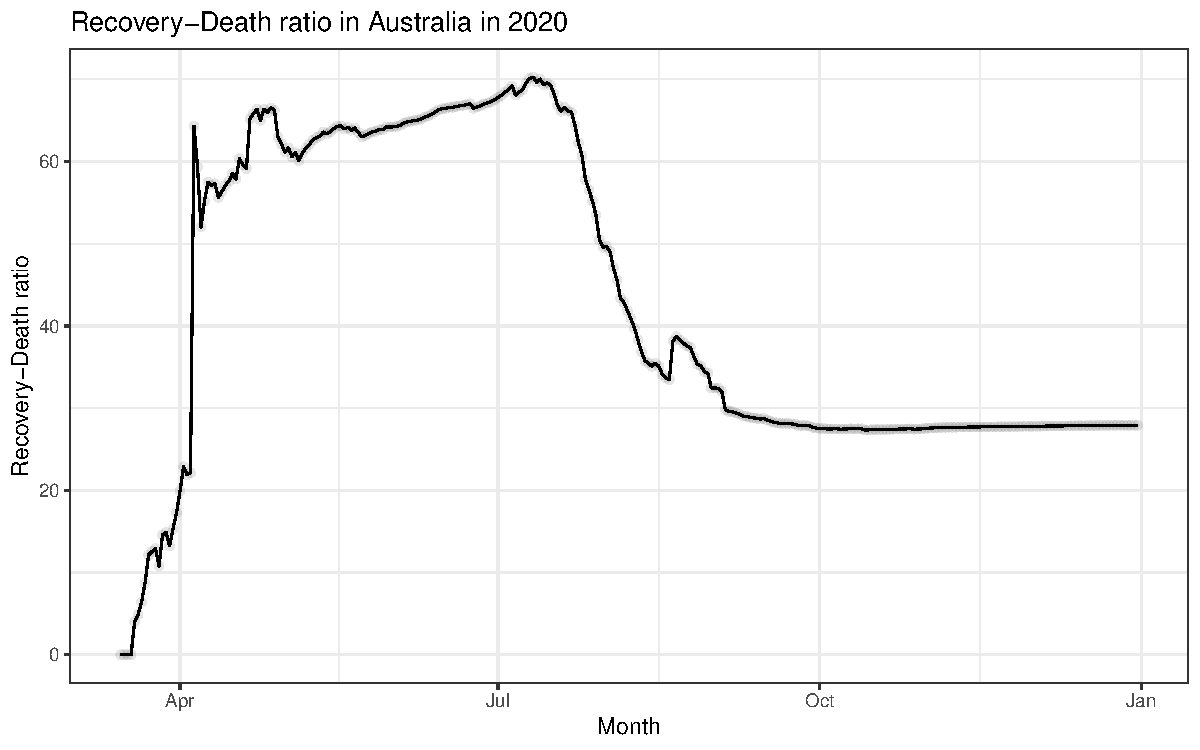
\includegraphics{report_files/figure-latex/figrec3-1.pdf}
\caption{\label{fig:figrec3}Recovery-Death ratio in Australia in 2020}
\end{figure}

\hypertarget{analysis-5}{%
\subsection{Analysis}\label{analysis-5}}

Figure\ref{fig:figrec3} demonstrates the ratio of total recoveries and total deaths, which it kept zero in the earlier Mar because An early outbreak in March left the recovery rate at zero and the death rate rising. As the ratio continued rising until July(70), then it started dropping which means that as the active cases decreased, the recoveries number became less.

\section*{Transmission sources of daily cases in Australia}

\begin{figure}

{\centering 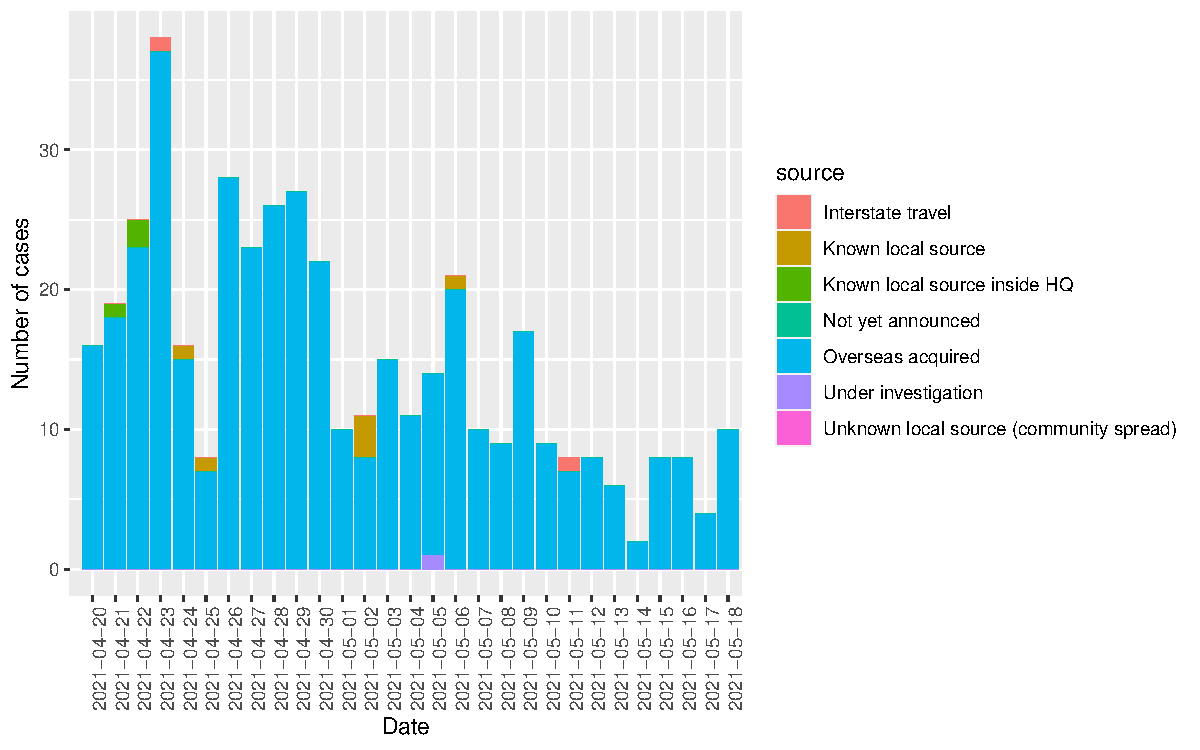
\includegraphics{report_files/figure-latex/tra-1} 

}

\caption{Transmission sources of daily cases 20 April 2021 - 18 May 2021}\label{fig:tra}
\end{figure}

The figure \ref{fig:tra} indicates that the most of transmissions were from overseas. Especially, there were more than 35 cases from overseas recorded and one case was due to the interstate travel in 23 April. Only One case is under investigation which has been recorded in 5 May.

Luckily, there are no more local community spread in Australia from 20 April 2021 to 18 May 2021.

\section*{Vaccination}

\hypertarget{vaccination-rates}{%
\subsection{Vaccination Rates}\label{vaccination-rates}}

\begin{figure}
\centering
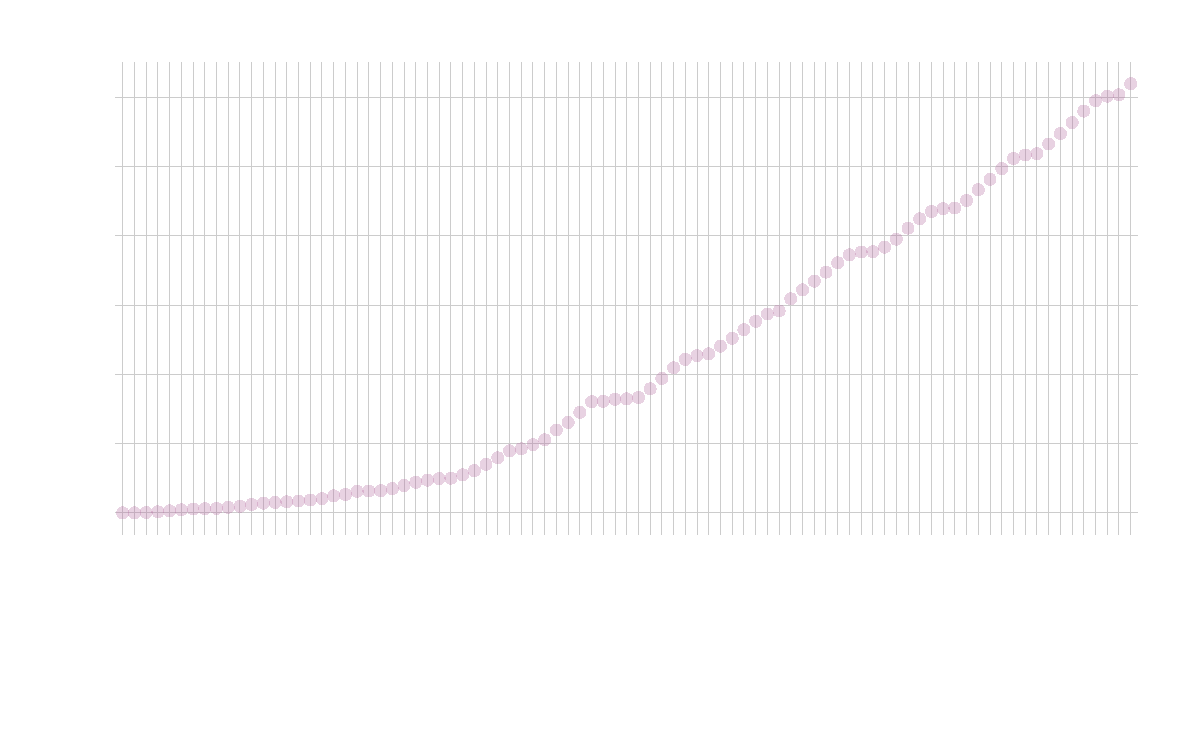
\includegraphics{report_files/figure-latex/FigRefplot-1.pdf}
\caption{\label{fig:FigRefplot}Vaccination Rates Over Time}
\end{figure}

The graph \ref{fig:FigRefplot} shows a general upward trend in vaccination, with the vaccination rate starting to show a faster increase in early April. The vaccination rate grows faster and faster over time. The number of vaccinations reached 12.39\% on May 18. The increase in vaccination rates illustrates the importance the government places on the outbreak.

\hypertarget{vaccination-coverage}{%
\subsection{Vaccination Coverage}\label{vaccination-coverage}}

\begin{figure}

{\centering 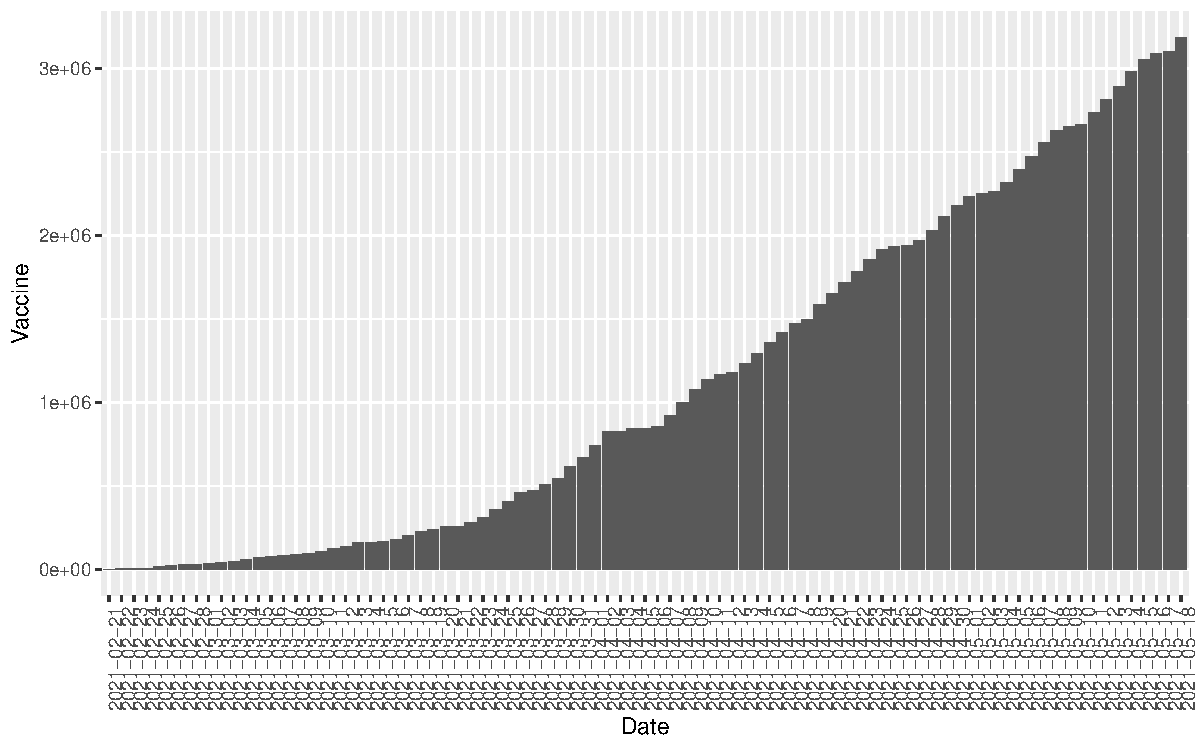
\includegraphics{report_files/figure-latex/FigRefz-1} 

}

\caption{Increase in vaccination coverage over time}\label{fig:FigRefz}
\end{figure}

We can see from the graph \ref{fig:FigRefz} that the number of inoculations continues to grow, from 20 people on February 21 to 3,183,324 people on May 18. The rate of growth has been accelerating since the beginning of April.

\hypertarget{conclusion-and-references}{%
\section{Conclusion and References}\label{conclusion-and-references}}

\hypertarget{conclusion}{%
\subsection{Conclusion}\label{conclusion}}

Given the analysis above, the number of the confirmed cases and their sources were very stable. Besides, with the high recovery rate and more people are taking the vaccines, it can be proved that the reactions Australian government made were effective.

\hypertarget{data}{%
\subsection{Data}\label{data}}

COVID-19 in Australia. (2021). Retrieved 18 May 2021, from \url{https://www.covid19data.com.au/}

\hypertarget{software}{%
\subsection{Software}\label{software}}

R Core Team (2020). R: A language and environment for statistical computing. R Foundation for Statistical Computing, Vienna, Austria. URL \url{https://www.R-project.org/}.

\hypertarget{packages}{%
\subsection{Packages}\label{packages}}

Alboukadel Kassambara (2020). ggpubr: `ggplot2' Based Publication Ready Plots. R package version 0.4.0. \url{https://CRAN.R-project.org/package=ggpubr}

Bob Rudis (2020). hrbrthemes: Additional Themes, Theme Components and Utilities for `ggplot2'. R package version 0.8.0. \url{https://CRAN.R-project.org/package=hrbrthemes}

C. Sievert. Interactive Web-Based Data Visualization with R, plotly, and shiny. Chapman and Hall/CRC Florida, 2020.

Hadley Wickham and Jennifer Bryan (2019). readxl: Read Excel Files. R package version 1.3.1. \url{https://CRAN.R-project.org/package=readxl}

Hao Zhu (2021). kableExtra: Construct Complex Table with `kable' and Pipe Syntax. R package version 1.3.4. \url{https://CRAN.R-project.org/package=kableExtra}

Müller, K. (2020). here: A Simpler Way to Find Your Files. R package version 1.0.1. \url{https://CRAN.R-project.org/package=here}

Pebesma, E., 2018. Simple Features for R: Standardized Support for Spatial Vector Data. The R Journal 10 (1), 439-446, \url{https://doi.org/10.32614/RJ-2018-009}

Richard Iannone, JJ Allaire and Barbara Borges (2020). flexdashboard: R Markdown Format for Flexible Dashboards. R package version 0.5.2. \url{https://CRAN.R-project.org/package=flexdashboard}

Simon Garnier, Noam Ross, Robert Rudis, Antônio P. Camargo, Marco Sciaini, and Cédric Scherer (2021). Rvision - Colorblind-Friendly Color Maps for R. R package version 0.6.0.

Wickham et al., (2019). Welcome to the tidyverse. Journal of Open Source Software, 4(43), 1686, \url{https://doi.org/10.21105/joss.01686}

Yihui Xie (2021). bookdown: Authoring Books and Technical Documents with R Markdown. R package version 0.22.

\printbibliography

\end{document}
